\chapter{EXPERIMENTAL RESULT}

\renewcommand{\headrulewidth}{0.5pt}
\renewcommand{\footrulewidth}{0.5pt}
\thispagestyle{plain}
\pagestyle{fancy}
\fancyhf{}
\fancyhead[L]{\textbf{CHAPTER 4}}
\fancyhead[R]{\textbf{DROWSINESS DETECTION AND ALERT SYSTEM IN THE CAR}}
\raggedright
\fancyfoot[L]{From: Nguyen Van Anh Tuan}
\fancyfoot[R]{Page \thepage}

\justifying

\section{Realistic Model}
    \begin{figure}[H]
        \centering
        \includegraphics[width=0.6\linewidth]{img/Hardware.png}
        \caption{Drowsiness detection model}
    \end{figure}
\section{Result}
    \begin{figure}[H]
        \centering
        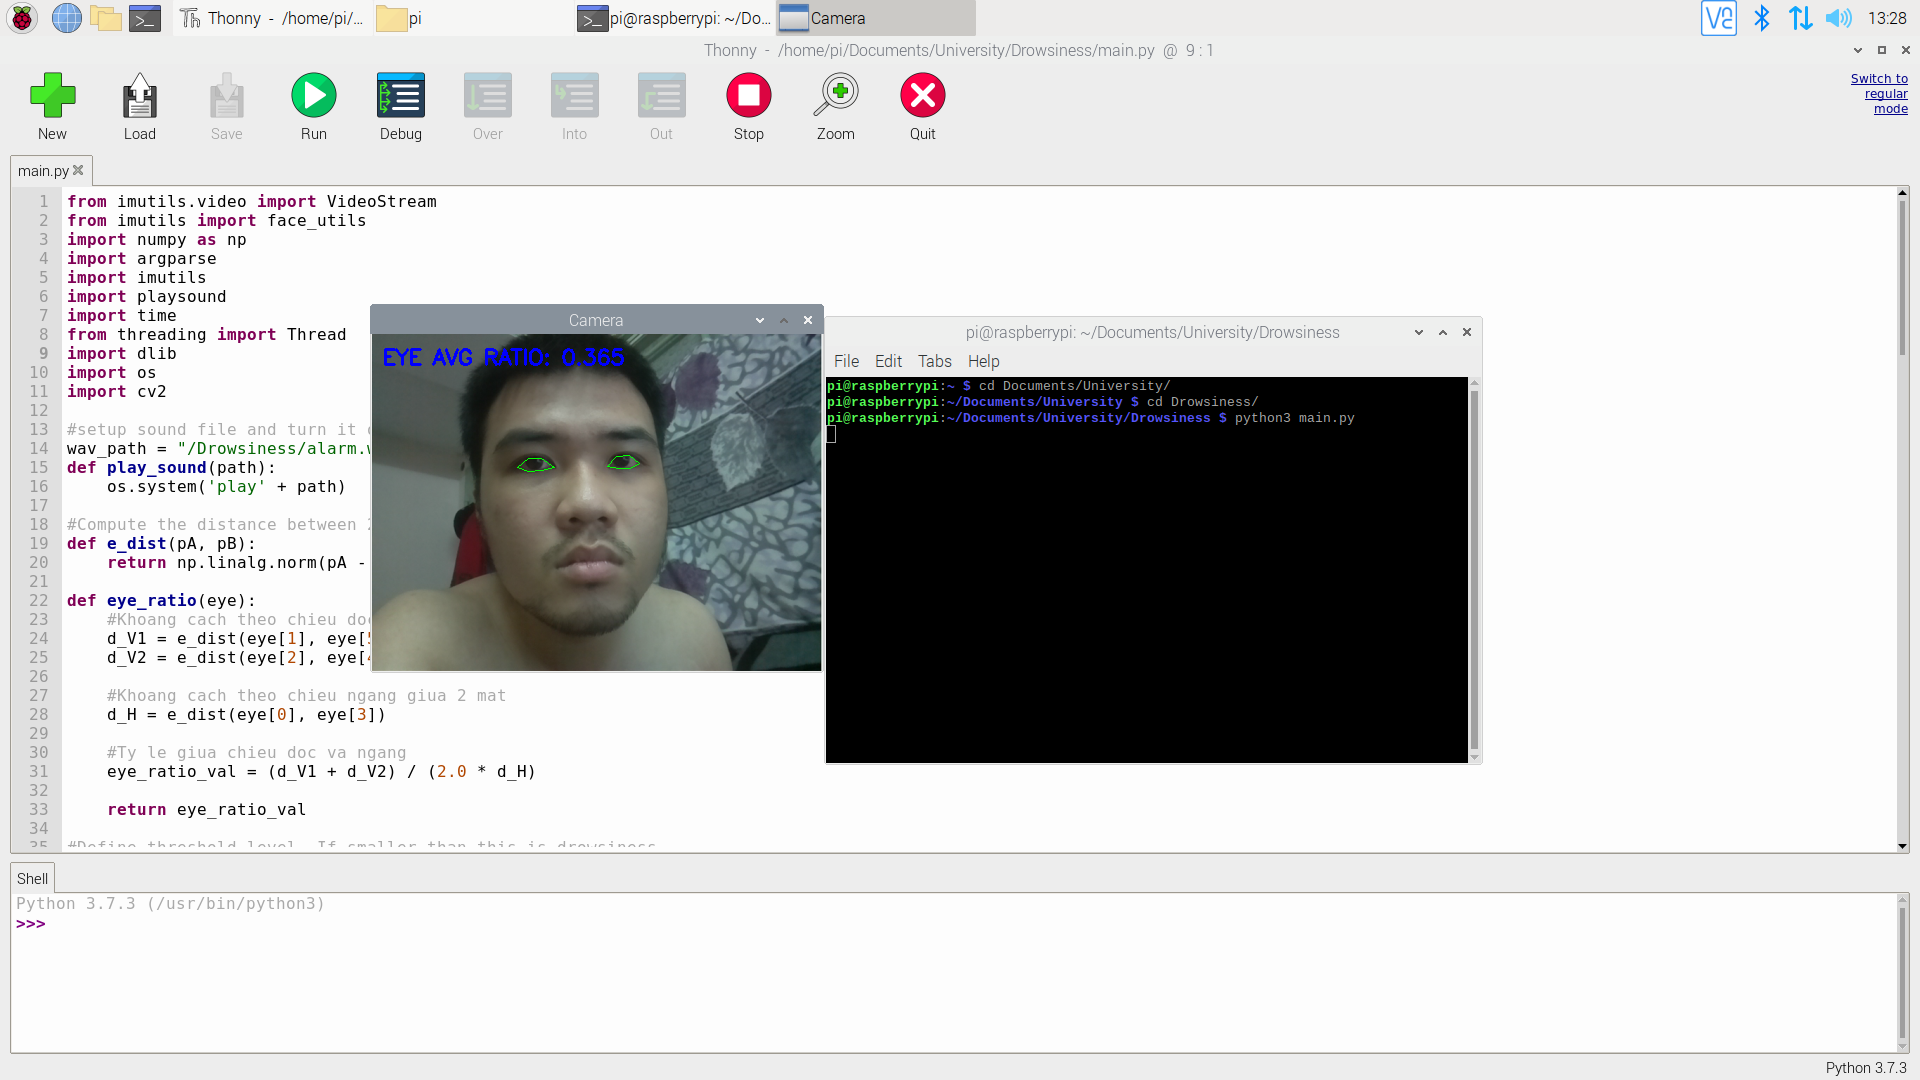
\includegraphics[width=0.8\linewidth]{img/run.png}
        \caption{Eye aspect ratio}
    \end{figure}
    In this picture, I tested the results when I was opening my eyes with an aspect ratio of 0.365 by the formula EAR (2.9)
    \begin{figure}[H]
        \centering
        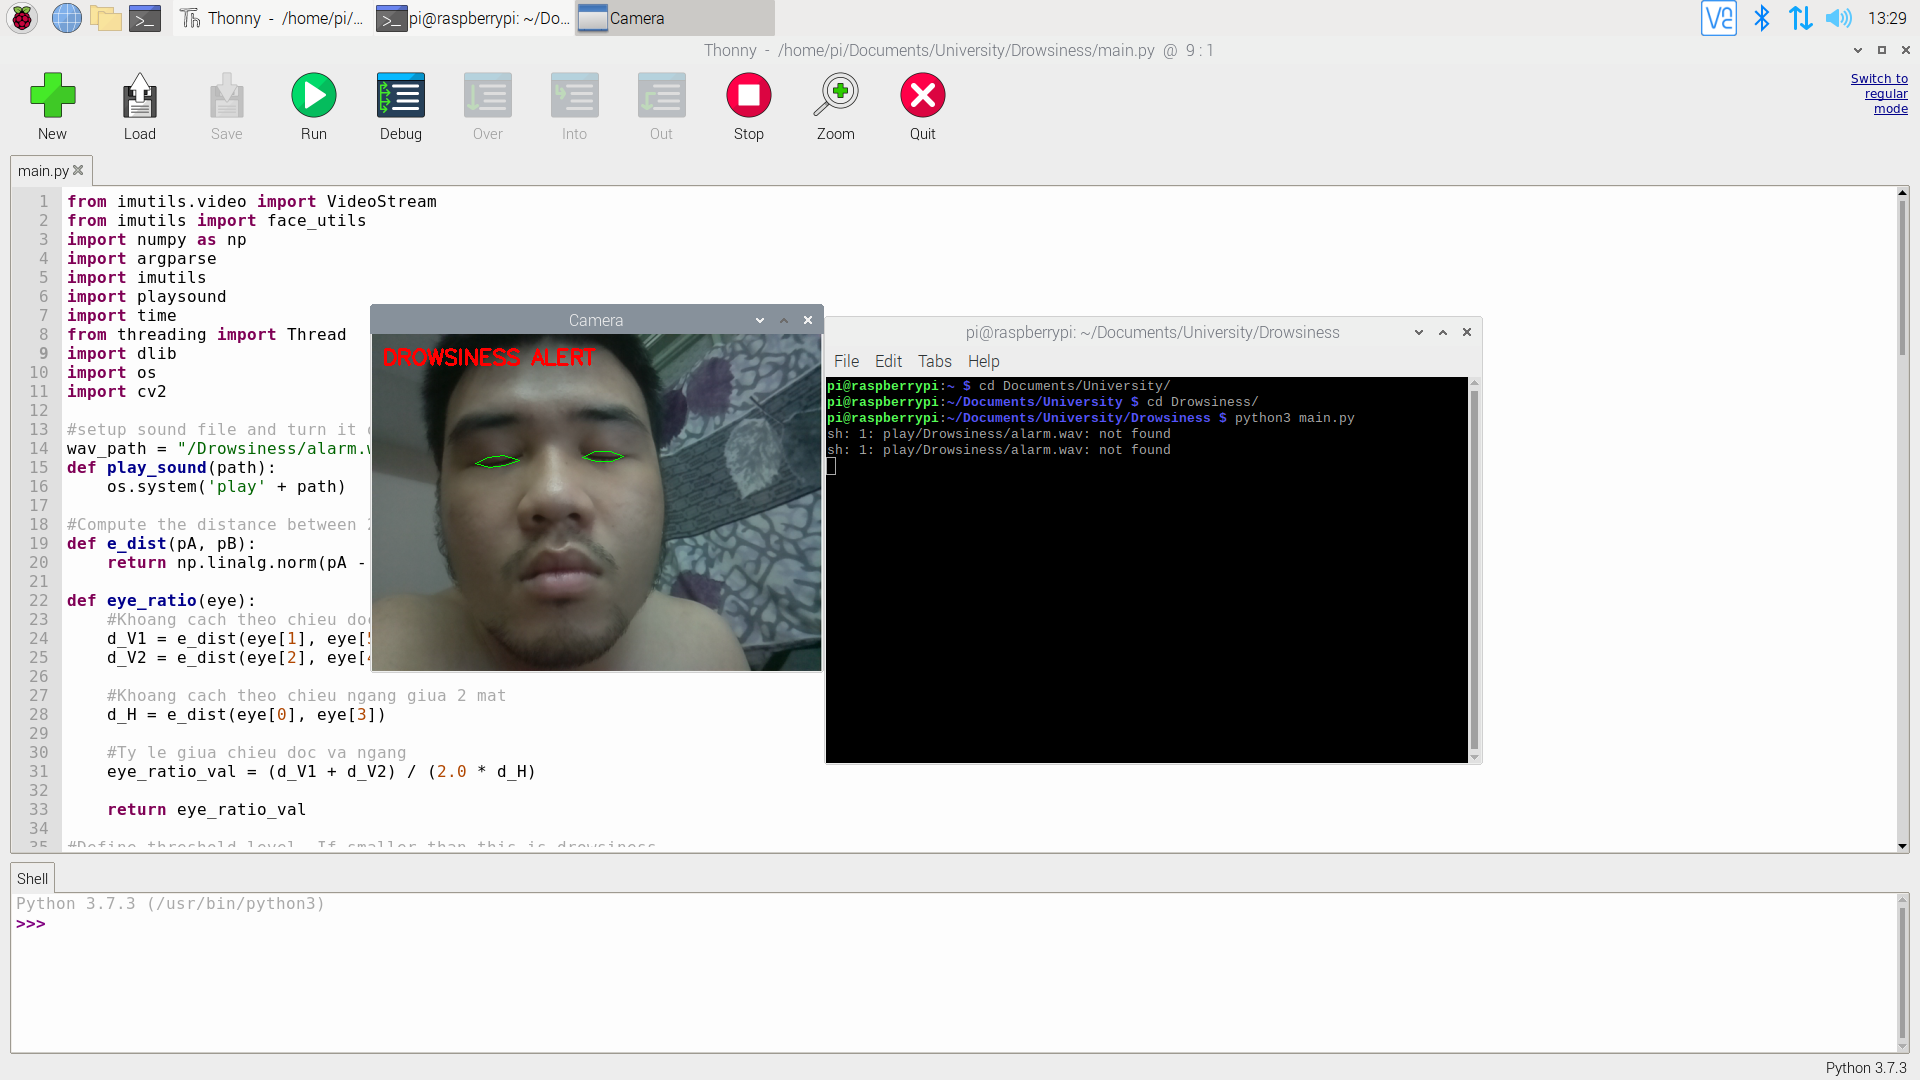
\includegraphics[width=0.8\linewidth]{img/result.png}
        \caption{Drowsiness detected}
    \end{figure}
    In case when the eye aspect ratio is too low (eyes are closed), there will be doze warning on screen and also in the speaker.